\documentclass{article}
\usepackage[utf8]{inputenc}
\usepackage{amsmath}
\usepackage[dvipsnames]{xcolor}
\usepackage{pgfplots}
\pgfplotsset{width=7cm,compat=1.3}
\usepackage{pgfplotstable}
\pgfplotsset{select coords between index/.style 2 args={
    x filter/.code={
        \ifnum\coordindex<#1\def\pgfmathresult{}\fi
        \ifnum\coordindex>#2\def\pgfmathresult{}\fi
    }
}}
\usepackage[utf8]{inputenc}
\usepackage{amsmath}
\usepackage{xcolor}

\begin{document}

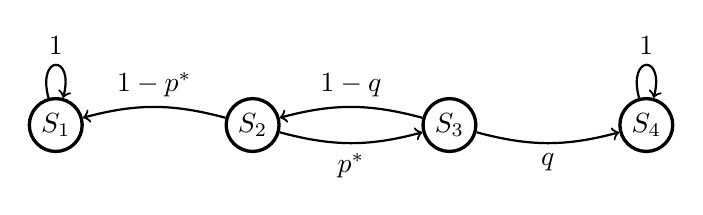
\begin{tikzpicture}
\def\xstep{2.5}
\def\bend{15}


\foreach \i in {1,...,4}{
\node[very thick, draw=black, circle, inner sep=2] (S\i) at (\i*\xstep, 0) {$S_{\i}$};
}

\draw[->, thick, bend right=\bend] (S2) to node[above]{$1-p^*$} (S1);
\draw[->, thick, bend right=\bend] (S2) to node[below]{$p^*$} (S3);

\draw[->, thick, bend right=\bend] (S3) to node[above]{$1-q$} (S2);
\draw[->, thick, bend right=\bend] (S3) to node[below]{$q$} (S4);

\draw[->, thick, loop above] (S1) to node[above]{$1$} (S1);
\draw[->, thick, loop above] (S4) to node[above]{$1$} (S4);

\end{tikzpicture}

\end{document}